\documentclass[10pt,a4paper]{article}
\usepackage[utf8]{inputenc}
\usepackage[left=2cm,right=2cm,top=2cm,bottom=2cm]{geometry}
\usepackage[dvipsnames]{xcolor}
\usepackage[fleqn]{mathtools}
\usepackage{booktabs}
\usepackage{amsmath}
\usepackage{latexsym}
\usepackage{graphicx}
\usepackage{nccmath}
\usepackage{multicol}
\usepackage{listings}
\usepackage{tasks}
\usepackage{color}
\usepackage{float}
\usepackage{lipsum}
\usepackage{cite}
\definecolor{colorIPN}{rgb}{0.5, 0.0,0.13}
\definecolor{colorESCOM}{rgb}{0.0, 0.5,1.0}
\definecolor{colorGENERICO}{rgb}{0.1, 0.6, 1.5}
\graphicspath{ {imagenes/} }

\begin{document}
%#########################################################
\begin{titlepage}
	\centering
	{ \huge \bfseries \color{colorIPN}{Instituto Politécnico Nacional} \par}
	{ \Large \bfseries  \color{colorESCOM}{Escuela Superior de Cómputo} \par }
	\vspace{1cm}
	{\huge\Large \color{colorIPN}{Técnologias para el Desarrollo de Aplicaciones Web}.\par}
	\vspace{1.5cm}
	{\huge\Large  \color{colorESCOM}{Práctica 2: Servlet y JDBC}\par}
		\vspace{2cm}
	{\Large\itshape \color{colorIPN}{Profesor: M. en C. José Asunción Enríquez Zárate}\par} \hfill \break
	\vspace{2cm}
	{\Large\itshape \color{colorIPN}{Alumno: Ulises Gómez Molina}\par} \hfill \break
	{\Large\itshape \color{colorIPN}{ulises21.uligom@gmail.com}\par} \hfill \break
	{\Large\itshape \color{colorIPN}{4CM2} \par}
	\vfill
	{\large \color{colorIPN}{\today}\par} 
	\vfill
\end{titlepage}

\renewcommand\lstlistingname{Quelltext} 


\lstset{ 
	language=Java,
	basicstyle=\small\sffamily,
	numbers=left,
	numberstyle=\tiny,
	frame=tb,
	tabsize=4,
	columns=fixed,
	showstringspaces=false,
	showtabs=false,
	keepspaces,
	commentstyle=\color{Violet},
	keywordstyle=\color{colorIPN} \bfseries,
	stringstyle=\color{colorESCOM}
}

\settasks{
	counter-format=(tsk[r]),
	label-width=4ex
}
\tableofcontents 
\pagebreak
\pagenumbering {arabic}

\pagebreak

%################################################
\section{\color{colorIPN}{Introducción}}
\normalsize{
Tan pronto como la Web se empezó a usar para proporcionar servicios, los
proveedores de éstos reconocieron la necesidad de contenido dinámico. Los Applets,
uno de los primeros intentos de conseguirlo, se concentran en el uso de la plataforma
del cliente para proporcionar al usuario este contenido dinámico.
\\
Al mismo tiempo, los desarrolladores también investigaron el uso del servidor
para lograr este propósito. Inicialmente, los scripts Common Gateway Interface (CGI)
fueron la principal tecnología utilizada para generar contenido dinámico. Aunque
ampliamente usados, la tecnología de scripts CGI tenía algunos inconvenientes,
incluyendo dependencia de la plataforma y falta de escalabilidad. Para solventar estas
limitaciones, la tecnología de Servlets Java se creó como un medio portable para
proporcionar contenido dinámico orientado al usuario.  Los componentes Web se ejecutan gracias a los servicios de una plataforma de ejecución llamada contenedor Web. Un contenedor Web proporciona servicios como entrega de peticiones, seguridad, concurrencia, y gestión de ciclos de vida. También
proporciona a los componentes Web acceso a las APIs. 
\\
La siguiente práctica ejemplifca el uso de servelts y JDBC, a traves de una aplicación Web para
controlar las categorías de productos, proporcionando una Web Gui para realizar las funcionalidades CRUD (Create-Read-Update-Delete) y así tener un mejor manejo de la información.

}

\section{\color{colorIPN}{Definiciones}}
\subsection{\color{colorESCOM}{Servlet}}
\normalsize{
Los Java Servlets son programas que se ejecutan en un servidor Web o de aplicaciones y actúan como una capa intermedia entre las peticiones procedentes de un navegador Web u otro cliente HTTP y el servidor.
entre las peticiones procedentes de un navegador Web u otro cliente HTTP y las bases de datos o aplicaciones en el servidor HTTP.
bases de datos o aplicaciones en el servidor HTTP.
Mediante los Servlets, puede recopilar datos de los usuarios a través de formularios de páginas web, presentar
registros de una base de datos u otra fuente, y crear páginas web dinámicamente.
\\
\\
Los Java Servlets requieren de un intérprete compatible con la especificación Java Servlet y pueden crearse utilizando los paquetes javax.servlet y javax.servlet.http,
que forman parte estándar de la edición empresarial de Java, una versión ampliada de la
biblioteca de clases Java que da soporte a proyectos de desarrollo a gran escala.
Estas clases implementan las especificaciones Java Servlet y JSP.
Los Java Servlets se crean y compilan como cualquier otra clase Java. Después de
de instalar los paquetes servlet y añadirlos al Classpath de tu ordenador, puedes compilar
servlets con el compilador Java del JDK o con cualquier otro compilador actual.
\\
\\
En el mercado existen varios servidores web compatibles con servlets. Algunos servidores
son de descarga gratuita y Tomcat es uno de ellos.
Apache Tomcat es una implementación de software de código abierto de las tecnologías Java Servlet y Java
Servidor de Páginas Java y puede actuar como un servidor independiente para probar servlets y
puede integrarse con el servidor web de Apache.

}
\subsection{\color{colorGENERICO}{JDBC}}
\normalsize{
JDBC son las siglas de Java Database Connectivity (conectividad de bases de datos de Java), una API Java estándar para la conectividad independiente de bases de datos entre el lenguaje de programación Java y una amplia gama de bases de datos.
\\
La biblioteca JDBC incluye API para cada una de las tareas que se mencionan a continuación y que suelen asociarse al uso de bases de datos.
asociadas con el uso de bases de datos.
\begin{itemize}
\item{Establecer una conexión con una base de datos.}
\item{Creación de sentencias SQL o MySQL.}
\item{Ejecución de consultas SQL o MySQL en la base de datos.}
\item{Visualización y modificación de los registros resultantes.}
\end{itemize}

Fundamentalmente, JDBC es una especificación que proporciona un conjunto completo de interfaces que permite acceso portátil a una base de datos subyacente. Java puede utilizarse para escribir diferentes tipos de ejecutables, tales como:
\begin{itemize}
\item Aplicaciones Java
\item Applets Java
\item Servlets Java
\item Java ServerPages (JSP)
\item Enterprise JavaBeans (EJB).
\end{itemize}


Todos estos ejecutables pueden utilizar un controlador JDBC para acceder a una base de datos y aprovechar los datos almacenados.
los datos almacenados.
JDBC proporciona las mismas capacidades que ODBC, permitiendo que los programas Java contengan código independiente de la base de datos.
\\
\\

}

\normalsize{
La API JDBC proporciona las siguientes interfaces y clases:
\begin{itemize}
\item \textbf{DriverManager}: Esta clase gestiona una lista de controladores de bases de datos. Relaciona las peticiones de conexión
conexión de la aplicación java con el controlador de base de datos adecuado utilizando
subprotocolo de comunicación. El primer driver que reconozca un determinado subprotocolo
bajo JDBC será utilizado para establecer una Conexión a la base de datos.

\item \textbf{Controlador}: Esta interfaz maneja las comunicaciones con el servidor de base de datos. Rara vez
interactuará directamente con los objetos Driver en muy raras ocasiones. En su lugar, se utiliza DriverManager. Los controladores JDBC son archivos de biblioteca Java con la extensión .jar utilizados por todas las aplicaciones Java para conectarse a la base de datos. Normalmente, son proporcionados por la misma compañía que implementó el software MySql. DbSchema Tool ya incluye un controlador MySql, que se descarga automáticamente al conectarse a MySql.

\item \textbf{Conexión}: Esta interfaz con todos los métodos para contactar con una base de datos. El objeto connection
representa el contexto de comunicación, es decir, toda la comunicación con la base de datos es
a través del objeto de conexión.

\item \textbf{Sentencia}: Los objetos creados a partir de esta interfaz se utilizan para enviar las sentencias SQL a la base de datos. Algunas interfaces derivadas aceptan parámetros además de ejecutar
procedimientos almacenados.

\item \textbf{ResultSet}: Estos objetos contienen datos recuperados de una base de datos después de ejecutar una consulta SQL mediante objetos Statement.
consulta SQL utilizando objetos Statement. Actúa como un iterador para permitirle moverse a través de
sus datos.

\item \textbf{SQLException}: Esta clase maneja cualquier error que ocurra en una aplicación de base de datos
\end{itemize}
La API JDBC utiliza un gestor de controladores y controladores específicos de bases de datos para proporcionar una conectividad transparente con bases de datos heterogéneas.
transparente a bases de datos heterogéneas.
El gestor de controladores JDBC garantiza que se utilice el controlador correcto para acceder a cada fuente de datos.
El gestor de controladores puede admitir varios controladores simultáneos conectados a varias bases de datos.

}

\subsection{\color{colorGENERICO}{Conectores}}
\normalsize{
La arquitectura Java EE Connector define una arquitectura estándar para conectar
la plataforma Java EE a EIS heterogéneos. Algunos ejemplos de EIS son Enterprise
Planificación de Recursos Empresariales (ERP), procesamiento de transacciones (TP) de mainframe y sistemas de bases de datos.
\\
La arquitectura del conector define un conjunto de mecanismos escalables, seguros y transaccionales que permiten la integración de EIS.
escalables, seguros y transaccionales que permiten la integración de los EIS con servidores de aplicaciones1 y aplicaciones empresariales.
La arquitectura de conectores también define una interfaz de cliente común (CCI) para el acceso a los EIS. La CCI define una API cliente para interactuar con EIS heterogéneos.
La arquitectura de conectores permite a un proveedor de EIS proporcionar un adaptador de recursos estándar para su EIS. 
\\
\\
Un adaptador de recursos es un controlador de software a nivel de sistema que una aplicación Java utiliza para conectarse a un EIS heterogéneo.
por una aplicación Java para conectarse a un EIS. El adaptador de recursos se conecta a un
servidor de aplicaciones y proporciona conectividad entre el EIS, el servidor de aplicaciones
y la aplicación empresarial. El adaptador de recursos sirve como un adaptador de protocolo
que permite utilizar cualquier protocolo de comunicación EIS arbitrario para la conectividad.
Un proveedor de servidores de aplicaciones amplía su sistema una vez para admitir la arquitectura del conector
y se asegura una conectividad sin fisuras con múltiples EIS. Del mismo modo,
un proveedor de EIS proporciona un adaptador de recursos estándar que tiene la capacidad de
conectarse a cualquier servidor de aplicaciones compatible con la arquitectura de conectores.
section
}
\section{\color{colorIPN}{Desarrollo}}
\normalsize{
El diagrama de clases utilizado se muestra a continuación.
}
\subsection{\color{colorESCOM}{Clase Categoria}}
\normalsize
{
La clase Categoria es el pilar de nuestra práctica. Es una clase que nos permite crear objetos
de tipo Categoria cuya información será introducida a la base de datos. A continuación se muestran
los métodos setters y getters que representan a la clase.

}
\begin{lstlisting}
public class Categoria{
     
    private int idCategoria;
    private String categoria;
    private String descripcionCategoria;
    
     public Categoria()
     {
     }

    public int getIdCategoria() {
        return idCategoria;
    }

    public void setIdCategoria(int idCategoria) {
        this.idCategoria = idCategoria;
    }

    public String getCategoria() {
        return categoria;
    }

    public void setCategoria(String categoria) {
        this.categoria = categoria;
    }

    public String getDescripcionCategoria() {
        return descripcionCategoria;
    }

    public void setDescripcionCategoria(String descrpcionCategoria) {
        this.descripcionCategoria = descrpcionCategoria;
    }

    @Override
    public String toString() {
        StringBuilder sb = new StringBuilder();
        sb.append("Clave:").append(idCategoria).append("\n");
        sb.append("nombre:").append(getCategoria()).append("\n");
        sb.append("descripcion").append(descripcionCategoria).append("\n");
        return sb.toString();
    }
}

\end{lstlisting} \hfill

\subsection{\color{colorESCOM}{Presentación del CRUD}}
\normalsize{
CRUD es el acrónimo de "Crear, Leer, Actualizar y Borrar", que se usa para referirse a las funciones básicas en bases de datos o la capa de persistencia en un software.
\\
Lo que se realizó para la práctica es una interfaz que permita realizar estas funciones de una manera más sencilla para el manejo de las categorias de productos. 
\\
Para ello, creamos una clase en JAVA llamada "CategoriaDao", la cuál nos permitirá realizar las conexiones con la base de datos previamente creada. 
\\
Primeramente se necesita la conexión con la base de datos, para ello, se crea un metodo "ObtenerConexion", una vez que se haya hecho un enlace exitoso, se pueden programar las demas funciones con ayuda de los respectivos queries.
\\
Para lograr la conexión, nos apoyamos de la libreria \textbf{java.sql}, la que nos proporciona la clase Connection y la PreparedStatement.
\\
\\
}
\begin{lstlisting}
	private void obtenerConexion()
    {
        String usuario = "root";
        String clave ="ulises.123";
        String url = "jdbc:mysql://localhost:3306/Practica2";
        String driver = "com.mysql.cj.jdbc.Driver";
        try {
            Class.forName(driver);
            con= DriverManager.getConnection(url,usuario,clave);
        } catch (ClassNotFoundException | SQLException ex) {
            Logger.getLogger(CategoriaDAO.class.getName()).log(Level.SEVERE, null, ex);
            System.out.println("No se pudo conectar :c");
        }
    }
\end{lstlisting} \hfill


\subsubsection{\color{colorGENERICO}{Crear}}
\begin{lstlisting}
	     public void insertarCategoria(Categoria c) throws SQLException{
        PreparedStatement ps = null; //acceso a datos
        obtenerConexion();
        try{
            ps=con.prepareStatement(SQL_INSERTAR);//PREPARAR LA CONSULTA
            ps.setString(1, c.getCategoria());
            ps.setString(2,c.getDescripcionCategoria());
            ps.executeUpdate();
  
        }finally
        {
            if(ps != null) ps.close();
            if(con != null) con.close();
        }
    }
\end{lstlisting} \hfill

\subsubsection{\color{colorGENERICO}{Leer}}
\normalsize{
Leer los datos implica que se deben obtener tanto los datos completos de la base de datos
como los registros individuales, por lo que se crean las funciones para ambos casos. Cabe
recalcar que para ambos métodos, se requiere de otro método para obtener los resultados individuales, que, posteriormente, se agregarán a una lista de registros.
}

\begin{lstlisting}
	    public List mostrarTodo() throws SQLException
    {
        obtenerConexion();
        PreparedStatement ps= null;
        ResultSet rs = null;
        try{
            ps = con.prepareStatement(SQL_SELECT_ALL);
            rs= ps.executeQuery();
            List resultados = obtenerResultados(rs);
            if (resultados.size() >0) {
                return resultados;
            }
            else
            {
                return null;
            }
        }finally
        {
            if(rs!= null) rs.close();
            if(ps != null) ps.close();
            if(con != null) con.close();   
        }
    }
    
    
    public Categoria MostrarUno(Categoria c) throws SQLException{
        obtenerConexion();
        PreparedStatement ps= null;
        ResultSet rs = null;
        try{
            ps = con.prepareStatement(SQL_SELECT);
             ps.setInt(1, c.getIdCategoria());
            rs= ps.executeQuery();
            List resultados = obtenerResultados(rs);
            if (!resultados.isEmpty()) {
                return (Categoria) resultados.get(0);
            }
            else
            {
                return null;
            }
            }
        finally{
            if(rs!= null) rs.close();
            if(ps != null) ps.close();
            if(con != null) con.close(); 
        }
  
}
    
        private List obtenerResultados(ResultSet rs) throws SQLException{
       List resultados = new ArrayList();
       while(rs.next())
       {
           Categoria c = new Categoria();
           c.setIdCategoria(rs.getInt("idCategoria"));
           c.setCategoria(rs.getString("nombreCategoria"));
           c.setDescripcionCategoria(rs.getString("descripcion"));
           resultados.add(c);
       }
       
       return resultados;
    }

\end{lstlisting} \hfill

\subsubsection{\color{colorGENERICO}{Actualizar}}
\begin{lstlisting}
 public void actualizarCategoria(Categoria c) throws SQLException
    {
        obtenerConexion();
        PreparedStatement ps = null; //Prepara las consultas;
        try
        {
            ps= con.prepareStatement(SQL_UPDATE);
            ps.setString(1, c.getCategoria());
            ps.setString(2,c.getDescripcionCategoria());
            ps.setInt(3, c.getIdCategoria());
            ps.executeUpdate();
        }finally
        {
             if(ps != null) ps.close();
            if(con != null) con.close();      
        }
    }
\end{lstlisting} \hfill


\subsubsection{\color{colorGENERICO}{Borrar}}
\begin{lstlisting}
	     public void eliminarCategoria(Categoria c) throws SQLException
    {
        obtenerConexion();
        PreparedStatement ps = null; //Prepara las consultas;
        try
        {
            ps= con.prepareStatement(SQL_DELETE);
            ps.setInt(1, c.getIdCategoria());
            ps.executeUpdate();
        }finally
        {
             if(ps != null) ps.close();
            if(con != null) con.close();      
        }
    }
\end{lstlisting} \hfill

\subsection{\color{colorESCOM}{Formularios y validaciones}}
\normalsize{
Para la muestra de la página, se utilizó diferentes servelts para mostrar las funcionalidades del 
CRUD, sin embargo, las que nos interesa son aquellos que incluyen algún formulario para insertar algún 
registro a la base de datos, en este caso son Actualizar e Insertar
}
\subsubsection{\color{colorGENERICO}{Actualizar}}
\begin{lstlisting}
    protected void processRequest(HttpServletRequest request, HttpServletResponse response)
            throws ServletException, IOException {
response.setContentType("text/html;charset=UTF-8");
            try (PrintWriter out = response.getWriter()) {
            /* TODO output your page here. You may use following sample code. */
            out.println("<!DOCTYPE html>");
            out.println("<html>");
            out.println("<head>");
            out.println("<title>Hola mundo</title>");            
            out.println("<link href=\"https:
            //cdn.jsdelivr.net/npm/bootstrap@5.2.3/dist/css            
            /bootstrap.min.css\" rel=\"stylesheet\" 
            integrity=\"sha384rbsA2VBKQhggwzxH7pPCaAqO46MgnOM80zW1RWuH61DGLwZJEdK2Kadq2F9CUG65\" 
            crossorigin=\"anonymous\">");
            out.println("<script src='https:
            //cdn.jsdelivr.net/npm/bootstrap@5.2.3/dist/js/bootstrap.bundle.min.js' ></script>");
            out.println("<title>Servlet ActualizarCategoria</title>");            
            out.println("</head>");
            out.println("<body>");
          out.println("<form method=\"post\" class=\"form-register\" name\"formulario\">");
          
                    out.println("<div class=\"card\">");
           out.println("<div class='card-header text-center text-primary'>");
            out.println("<h1 class='card-title'>Modificar categoria...</h1>");
           out.println("</div>");
             out.println("<div class='card-body text-center text-primary'>");
            out.println("<h3>Nombre de la categoria</h3>");
            out.println("<input name=\"Nombre\" id=\"Nombre\" TYPE=\"TEXT\" 
            SIZE=\"50\" MAXLENGTH=\"50\">");
            out.println("<h3>Descripcion de la categoria</h3>");
            out.println("<input name=\"Descripcion\" id=\"Descripcion\" TYPE=\"TEXT\" 
            SIZE=\"50\" MAXLENGTH=\"50\">");
            out.println("</div>");          
            out.println("<div class='card-footer text-center'>");
            out.println("<input type=\"submit\" value=\"Enviar\" class='btn btn-success'>");
            
            out.println("<a href='Listado' class='btn btn-info'>Regresar al listado</a>");
            out.println("</div>");
            out.println("</div>");
            out.println("</form>");
            out.println("<script
             src=\"//cdnjs.cloudflare.com/ajax/libs/validate.js/0.13.1/validate.min.js\" 
             integrity=\"sha256-FtvY52LIDZ2/QHmDNay6PTYvLkRsZICHak0iJEAIBuM=\" 
            crossorigin=\"anonymous\"></script>");
            out.println("</body>");
            out.println("</html>");
        }
    }
    
    @Override
    protected void doPost(HttpServletRequest request, HttpServletResponse response)
            throws ServletException, IOException {
       //
             CategoriaDAO dao = new CategoriaDAO();
            Categoria c = new Categoria();
            int id=Integer.parseInt(request.getParameter("id"));
            c.setIdCategoria(id);
        String Nombre = request.getParameter("Nombre");
            String Descripcion = request.getParameter("Descripcion");
            c.setCategoria(Nombre);
            c.setDescripcionCategoria(Descripcion);
            try {
                dao.actualizarCategoria(c);
            } catch (SQLException ex) {
                Logger.getLogger(EliminarCategoria.class.getName()).log(Level.SEVERE, null, ex);
            }
       processRequest(request, response);
    }
\end{lstlisting} \hfill

\subsubsection{\color{colorGENERICO}{Agregar}}
\begin{lstlisting}
	  protected void processRequest(HttpServletRequest request, HttpServletResponse response)
            throws ServletException, IOException {
        response.setContentType("text/html;charset=UTF-8");
        try (PrintWriter out = response.getWriter()) {
            /* TODO output your page here. You may use following sample code. */
            out.println("<!DOCTYPE html>");
            out.println("<html>");
            out.println("<head>");
            out.println("<title>Hola mundo</title>");            
            out.println("<link href=\"https:
            //cdn.jsdelivr.net/npm/bootstrap@5.2.3/dist/css/bootstrap.min.css\" rel=\"stylesheet\" integrity=\"sha384-rbsA2VBKQhggwzxH7pPCaAqO46MgnOM80zW1RWuH61DGLwZJEdK2Kadq2F9CUG65\" 
            crossorigin=\"anonymous\">");
            out.println("<script src='https://cdn.jsdelivr.net/npm/bootstrap@5.2.3/
            dist/js/bootstrap.bundle.min.js' ></script>");
            out.println("<title>Servlet AgregarCategoria</title>");            
            out.println("</head>");
            out.println("<body>");
          out.println("<form method=\"post\" class=\"form-group\">");
          
          out.println("<div class=\"card\">");
           out.println("<div class='card-header text-center text-primary'>");
            out.println("<h1 class='card-title'>Agregar categoria...</h1>");
           out.println("</div>");
           
           out.println("<div class='card-body text-center text-primary'>");
            out.println("<h2>Nombre de la categoria</h2>");
            out.println("<input name=\"Nombre\" id=\"Nombre\" TYPE=\"TEXT\" 
            SIZE=\"50\" MAXLENGTH=\"50\">");
            out.println("<h2>Descripcion de la categoria</h2>");
            out.println("<input name=\"Descripcion\" id=\"Descripcion\" 
            TYPE=\"TEXT\" SIZE=\"50\" MAXLENGTH=\"50\">");
            out.println("</div>");          
            out.println("<div class='card-footer text-center'>");
            out.println("<input type=\"submit\" value=\"Enviar\"
             class='btn btn-success'>");
            out.println("<a href='Listado' class='btn btn-info'>Regresar al listado</a>");
            out.println("</div>");
            out.println("</div>");
            out.println("</body>");
            out.println("</html>");
        }
    }
    
    @Override
    protected void doPost(HttpServletRequest request, HttpServletResponse response)
            throws ServletException, IOException {
        CategoriaDAO dao = new CategoriaDAO();
            Categoria c = new Categoria();
        String Nombre = request.getParameter("Nombre");
            String Descripcion = request.getParameter("Descripcion");
            c.setCategoria(Nombre);
            c.setDescripcionCategoria(Descripcion);
            try {
                dao.insertarCategoria(c);
            } catch (SQLException ex) {
                Logger.getLogger(EliminarCategoria.class.getName()).log(Level.SEVERE, null, ex);
            }
       processRequest(request, response);
        processRequest(request, response);
    }
\end{lstlisting} \hfill


\subsection{\color{colorESCOM}{Resultados}}
\normalsize{
Los resultados obtenidos, se muestran a continuacion:
}
\begin{figure}[H]
	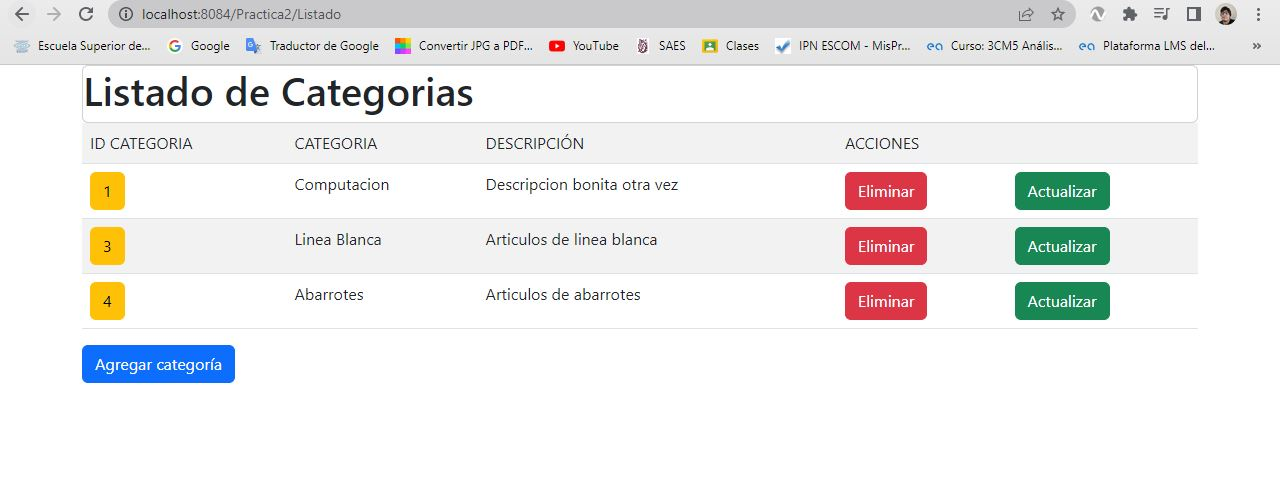
\includegraphics[scale=.54]{Imagenes/c1.jpg}
	\centering  
	\caption{Listado de todos los registros de la base de datos}
\end{figure} \hfill 

\begin{figure}[H]
	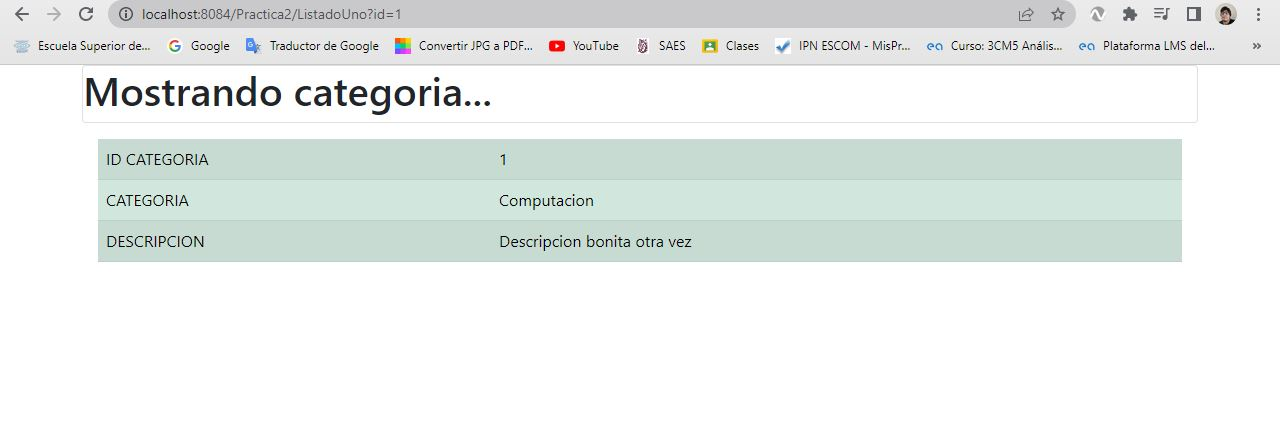
\includegraphics[scale=.54]{Imagenes/mostrarUno.jpg}
	\centering  
	\caption{Muestra de un solo registro}
\end{figure} \hfill 

\begin{figure}[H]
	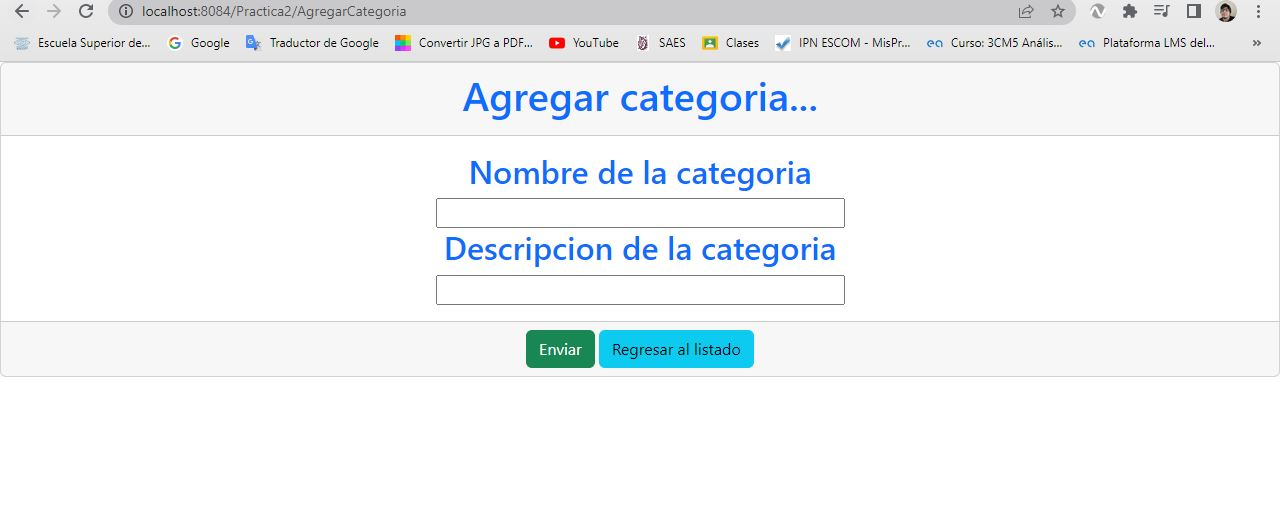
\includegraphics[scale=.54]{Imagenes/crear.jpg}
	\centering \linebreak 
	\caption{Agregar una categoria nueva}
\end{figure} \hfill 

\begin{figure}[H]
	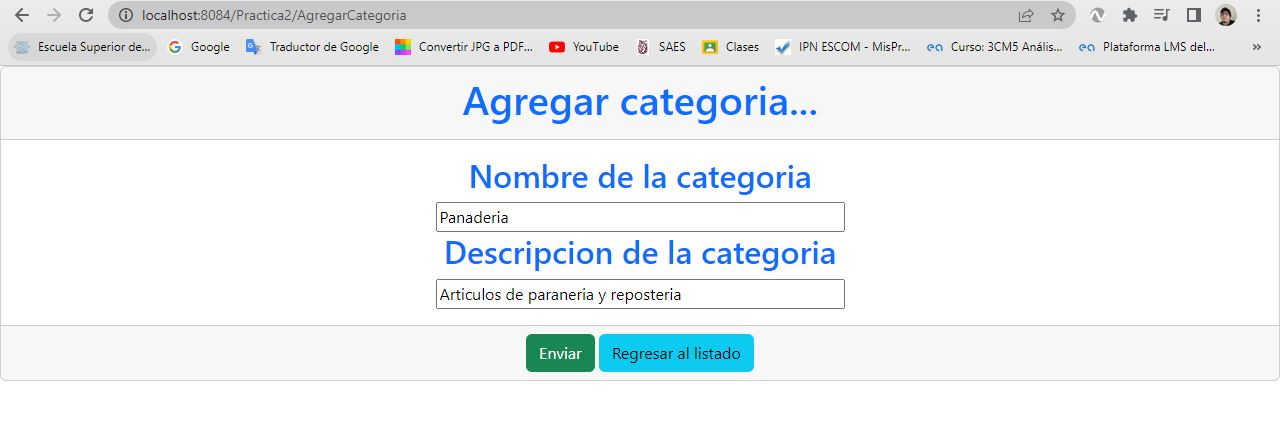
\includegraphics[scale=.54]{Imagenes/validacionAgregar.jpg}
	\centering \linebreak 
	\caption{Muestra de cómo se agrega una categoria nueva}
\end{figure} \hfill 

\begin{figure}[H]
	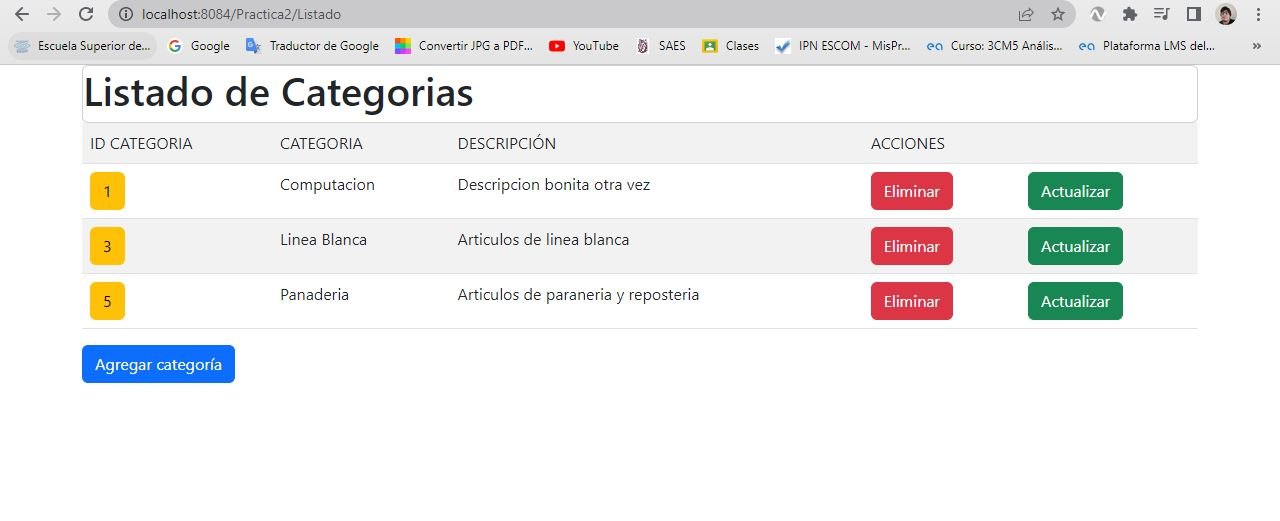
\includegraphics[scale=.54]{Imagenes/validacionAgregarMostrar.jpg}
	\centering \linebreak 
	\caption{Muestra de la adición de una nueva categría}
\end{figure} \hfill 

\begin{figure}[H]
	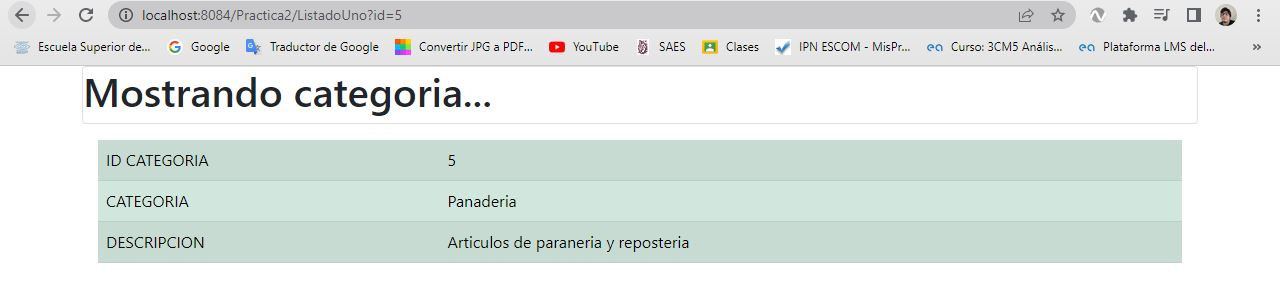
\includegraphics[scale=.54]{Imagenes/MostrarNuevo.jpg}
	\centering \linebreak 
	\caption{Muestra individual de la categoria agregada}
\end{figure} \hfill 

\begin{figure}[H]
	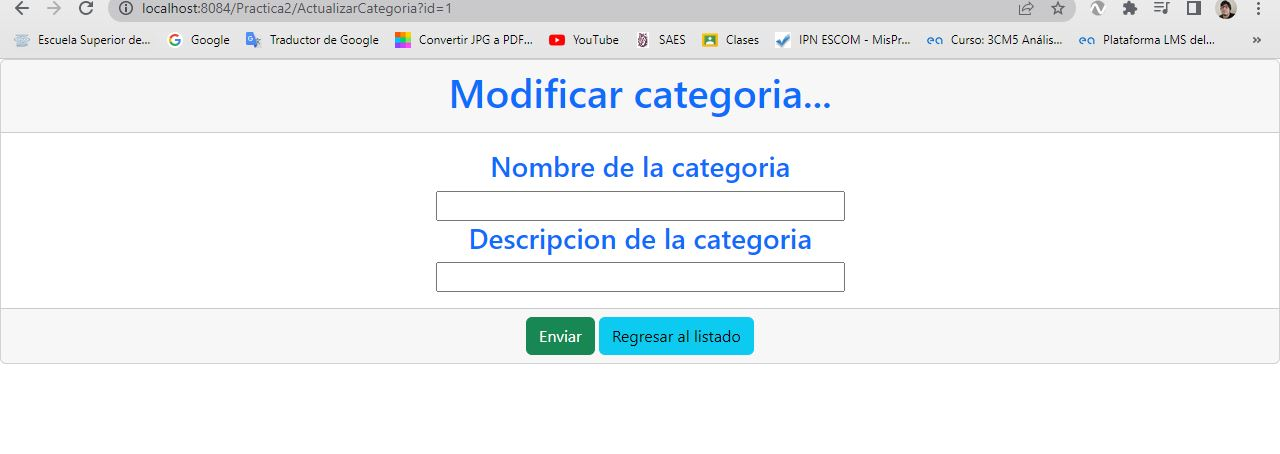
\includegraphics[scale=.54]{Imagenes/modificar.jpg}
	\centering 
	\caption{Modificar una categoria}
\end{figure}


\begin{figure}[H]
	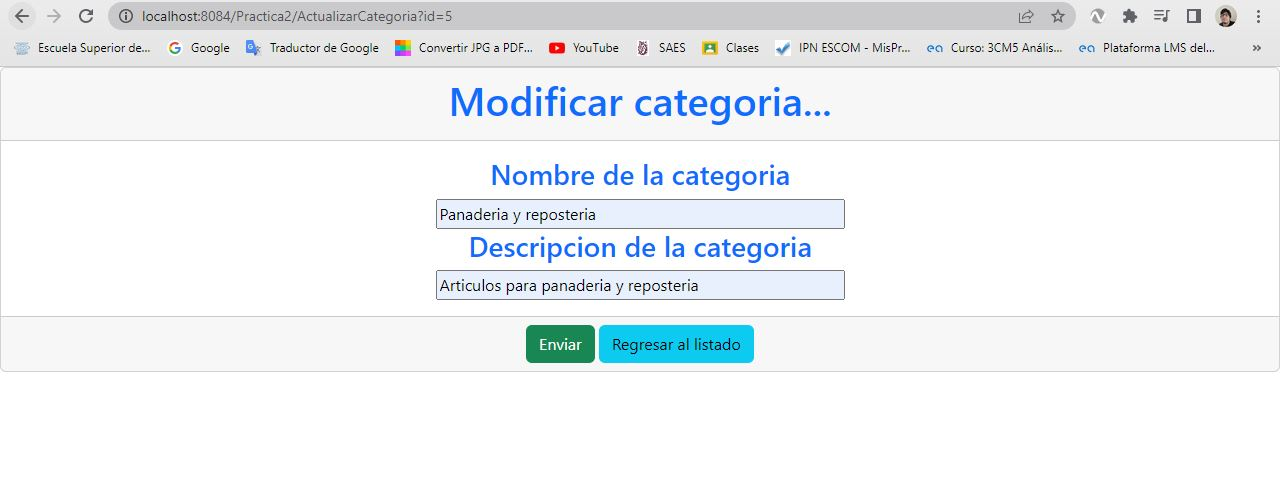
\includegraphics[scale=.54]{Imagenes/modificarValidacion.jpg}
	\centering \linebreak \linebreak 
	\caption{Muestra de cómo se modificar una categoria}
\end{figure} \hfill 

\begin{figure}[H]
	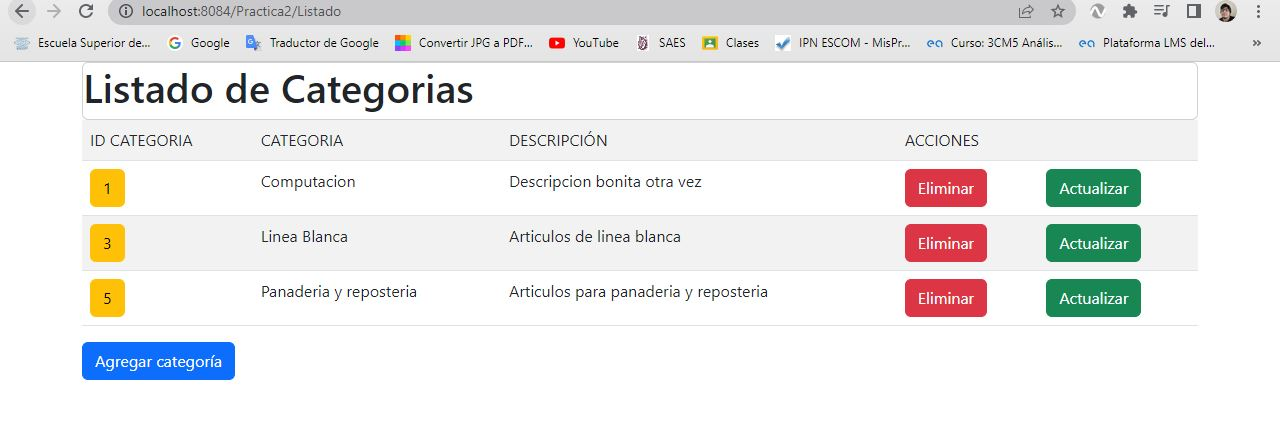
\includegraphics[scale=.54]{Imagenes/mostrarModificado.jpg}
	\centering \linebreak \linebreak 
	\caption{Muestra de la actualización de la categoria "Articulos de panaderia"}
\end{figure} \hfill 

\begin{figure}[H]
	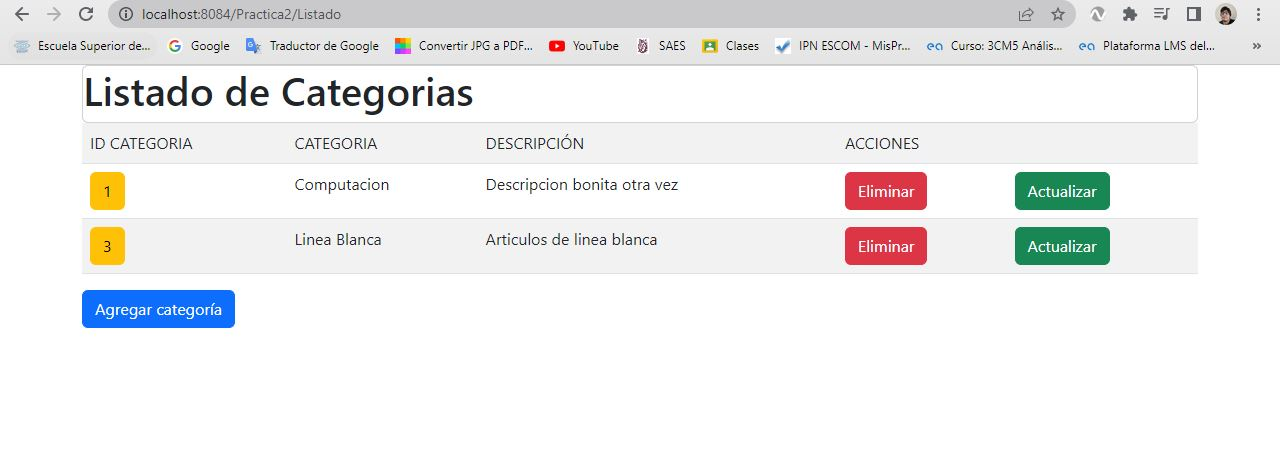
\includegraphics[scale=.54]{Imagenes/mostrarEliminar.jpg}
	\centering \linebreak \linebreak 
	\caption{Muestra el mensaje de eliminación de una categoria}
\end{figure} \hfill 

\section{\color{colorIPN}{Conclusiones}}
\normalsize
{
Los servlets son programas en Java que construyen o sirven páginas web. En esta práctica se pudo comprobar que los servlets pueden construir páginas dinámicas, basadas en diferentes fuentes variables: datos proporcionados por el usuario o que extraigan información de bases de datos.
\\
El manejo de servlets implica trabajar con ciertas tecnologías y aunque sean muy variadas, se pudo trabajar con:
}

\begin{itemize}
\item Un servidor web que dé soporte a servlets / JSP (contenedor de servlets y páginas JSP). En este caso se utilizó Apache Tomcat en su version 9.0, que requiere la dependencia javax recuperada del Maven
repository.
\item Las librerías necesarias para trabajar con servlets. Normalmente vienen en ficheros JAR en un directorio lib del servidor (common/lib en Tomcat): servlet.jar (con la API para servlets), y jsp.jar, jspengine.jar o jasper.jar (para JSP). Al desarrollar nuestra aplicación, deberemos incluir las librerías necesarias en el CLASSPATH para que compilen los ficheros.
\item Frameworks para el diseño de la web GUI, para esta práctica se usó el CSS proporcionado por Bootstrap, aunque se pudieron haber utilizado algún otro.
\item Un sistema de base de datos. Para esta práctica se hizo uso de Mysql Workbench para la creación y poblado de la base de datos utilizada.
\end{itemize}

\normalsize
{
Los Servlets Java nos permiten fácilmente hacer muchas cosas que son difíciles o imposibles con CGI normal. Por algo, los servlets pueden hablar directamente con el servidor Web. Esto simplifica las operaciones que se necesitan para buscar imágenes y otros datos almacenados en situaciones estándar y también pueden compartir los datos entre ellos, haciendo las cosas útiles como almacenes de conexiones a bases de datos fáciles de implementar. También pueden mantener información de solicitud en solicitud, simplicando cosas como seguimiento de sesión y el caché de cálculos anteriores.
Portable. Los Servlets están escritos en Java y siguen un API bien estándarizado. Consecuentemente, los servlets escritos, digamos en el servidor I-Planet Enterprise, se pueden ejecutar sin modificarse en Apache, Microsoft IIS, o WebStar. Los Servlets están soportados directamente o mediante plug-in en la mayoría de los servidores Web.
}
\section{\color{colorIPN}{Referencias Bibliográficas}}
\color{colorESCOM}{
	\begin{itemize}
	\item  Tyson, W.is: J.B.M. and Tyson, M. (2022) What is JDBC? introduction to java database connectivity, InfoWorld. JavaWorld. Available at: https://www.infoworld.com/article/3388036/what-is-jdbc-introduction-to-java-database-connectivity.html (Accessed: January 4, 2023). 
	\item The java EE 5 tutorial (2007) What Is a Servlet? - The Java EE 5 Tutorial. Available at: https://docs.oracle.com/javaee/5/tutorial/doc/bnafe.html (Accessed: January 7, 2023). 
	\item What is JDBC? (no date) IBM. Available at: https://www.ibm.com/docs/en/informix-servers/12.10?topic=started-what-is-jdbc (Accessed: January 7, 2023). 
	\end{itemize}




\end{document}
